\section{Signal performance of a detector}


\subsection{Signal response}

A particle is detected if it passes through our detector and leaves some
energy behind. These detections end up as a digitized list of numbers
with a timestamp. However, before a particle signal ends up in its
digital form it passes through the various parts of the detector. Not
all parts perfectly transport the particle signal. These effects, which
prevent the detector from having perfect timing and particle counting
will be outlined. These also serve as probability distributions that are
used in detector simulations.


\subsection{Energy loss and light production}

Particles loose energy in the detector because of interactions with the
polyvinyltoluene in the scintillator. Ionization and Bremsstrahlung and
the main sources of energy loss for energetic charged particles
(electrons, muons). The energy is transferred to anthracene molecules which emit light that

This formula gives the stopping power, the amount of energy
lost by the particle per \SI{}{\gram\centi\meter\square} of the material
it passes through. However, the interactions in which the particles
loose energy is a statistical process, so the energy loss is not a fixed
number but a distribution. (figure...)

The scintillator is \SI{2}{\centi\meter} thick, however, most particles
have a longer path through the detector because they enter it at an
angle. The path can be shorter if the particle passes through one of the
edges of the scintillator, but due to the large area of the detector
relative to its thickness the chance of that happening is low. The
amount of energy deposited by the particle going through the detector is
described by the Bethe-Bloch formula. 

According to the specifications the amount of light produced in a
scintillator as a function of temperature should be constant between
\SI{-60}{\degreeCelsius} and \SI{20}{\degreeCelsius}. At
\SI{60}{\degreeCelsius} the light output is decreased by
\SI{5}{\percent} relative to the output at \SI{20}{\degreeCelsius}.
Temperature in a skibox can rise above the local outside temperature
when the sun shines upon it. Temperature loggers have measured
differences of over \SI{10}{\degreeCelsius} above the local outside
temperature. Rarely but sometimes the temperature in the Netherlands can
reach \SI{40}{\degreeCelsius}, so on such occasions the efficiency of
the scintillator might be \SI{3.75}{\percent} below nominal. Given the
rare occurrence of such extremely high temperatures and the small effect
this is ignored in the analysis and simulations.


\subsubsection{Gammas}

\todo{Signals in detector from gammas}

Energetic photons can also deposit energy in the scintillator due to
Compton scattering and pair creation. However, the cross sections for
these interactions is very low. A \SI{1}{\mega\electronvolt} photon  has
a mean free path greater than \SI{10}{\centi\meter}, which increases
further for higher energy photons, see fig [By Jos/Tom]. Despite the low
detection chance, the large number of photons in an air shower makes
them statistically relevant.


\subsection{Light transmission}

Because of the geometry of the detector the position of the scintillator
that the particle goes through is significant. The light emitted along
the path of the particle is transmitted in random directions. Depending
on the angle at which the emitted photons hit the outer edges of the
scintillator there is a chance that they will be reflected back or leave
the scintillator. The entire detector is wrapped in aluminium foil 
to reflect those photons back into the scintillator. To
detect the photons they need to hit the windows of \pmt. To get to the
\pmt they need to pass from the scintillator through a layer of optical
glue, the light guide, another layer of optical glue, a small piece of
light guide, and finally a layer of optical tape to reach the \pmt.
During this many photons will be reflected a number of times. For
\SI{1}{\mip} approximately 30000 photons [check.] are emitted, most will
not make it to the \pmt.

A 2D Monte Carlo simulation performed by Jos Steijger which tracked
photons from emission until they either reach the \pmt or leave the
detector (ignoring the aluminium foil) gives transmission efficiency
information at any location in the scintillator.

Coincidence tests using a small (\SI[product-units = repeat]{1 x
1}{\centi\meter}) scintillator with a \pmt and a normal \hisparc
detector provided verification of this simulation. By moving the small
detector over the large scintillator they will also trigger on single
muons passing through both detectors. This makes it possible to check
the efficiency at a specific point of the detector.

In the simulations we use the Bethe Bloch, energy straggling, Landau
distribution convoluted with the efficiency modelled by Jos as
distribution which can be scaled by cosine of angle of incidence.

\begin{figure}
    \centering
    % \usepackage{tikz}
% \usetikzlibrary{arrows}
% \usepackage{pgfplots}
% \pgfplotsset{compat=1.3}
% \usepackage[detect-family]{siunitx}
% \usepackage[eulergreek]{sansmath}
% \sisetup{text-sf=\sansmath}
% \usepackage{relsize}
%
\tikzsetnextfilename{externalized-signal_efficiency}
\pgfkeysifdefined{/artist/width}
    {\pgfkeysgetvalue{/artist/width}{\defaultwidth}}
    {\def\defaultwidth{ .67\linewidth }}
%
%
\begin{sansmath}
\begin{tikzpicture}[
        font=\sffamily,
        every pin/.style={inner sep=2pt, font={\sffamily\smaller}},
        every label/.style={inner sep=2pt, font={\sffamily\smaller}},
        every pin edge/.style={<-, >=stealth', shorten <=2pt},
        pin distance=2.5ex,
    ]
    \begin{axis}[
            axis background/.style={  },
            xmode=normal,
            ymode=normal,
            width=\defaultwidth,
            axis equal=false,
            %
            title={  },
            %
            xlabel={ Signal strength [\si{\mip}] },
            ylabel={ Counts },
            %
            xmin={  },
            xmax={  },
            ymin={ 0.0 },
            ymax={  },
            %
            xtick={  },
            ytick={  },
            %
            tick align=outside,
            max space between ticks=40,
            every tick/.style={},
            axis on top,
        ]

        






    
    % Draw series plot
    \addplot[no markers,solid,const plot] coordinates {
        (0.0, 0)
        (0.05, 0)
        (0.1, 0)
        (0.15, 0)
        (0.2, 0)
        (0.25, 0)
        (0.3, 0)
        (0.35, 0)
        (0.4, 0)
        (0.45, 5)
        (0.5, 62)
        (0.55, 121)
        (0.6, 205)
        (0.65, 277)
        (0.7, 349)
        (0.75, 397)
        (0.8, 476)
        (0.85, 563)
        (0.9, 604)
        (0.95, 676)
        (1.0, 635)
        (1.05, 681)
        (1.1, 582)
        (1.15, 549)
        (1.2, 505)
        (1.25, 471)
        (1.3, 411)
        (1.35, 365)
        (1.4, 344)
        (1.45, 292)
        (1.5, 235)
        (1.55, 184)
        (1.6, 152)
        (1.65, 145)
        (1.7, 112)
        (1.75, 122)
        (1.8, 103)
        (1.85, 83)
        (1.9, 86)
        (1.95, 58)
        (2.0, 47)
        (2.05, 43)
        (2.1, 32)
        (2.15, 17)
        (2.2, 10)
        (2.25, 1)
        (2.3, 0)
        (2.35, 0)
        (2.4, 0)
        (2.45, 0)
    };







    \end{axis}
\end{tikzpicture}
\end{sansmath}

    \caption{\captitle{Signal for a particle.} This distribution gives
             the signal from a single particles passing straight through
             a random location of the scintillator. The distribution
             scales with $\cos{\theta}^{-1}$.}
    \label{fig:signal_efficiency}
\end{figure}

Fokkema Fig 2.7, *2.8*, 2.9, 2.10.

Low efficiency: around ~2 \% across the detector, but not 0 \%!



\subsection{\pmt linearity}

Ideally the output of the \pmt grows is linear with the number of
particles in the detector. This is less important for a large number of
particles because the error on the number of particles also grows with
$\sqrt{n}$. Linearity is [currently] assumed in the analysis.

\begin{figure}
    \centering
    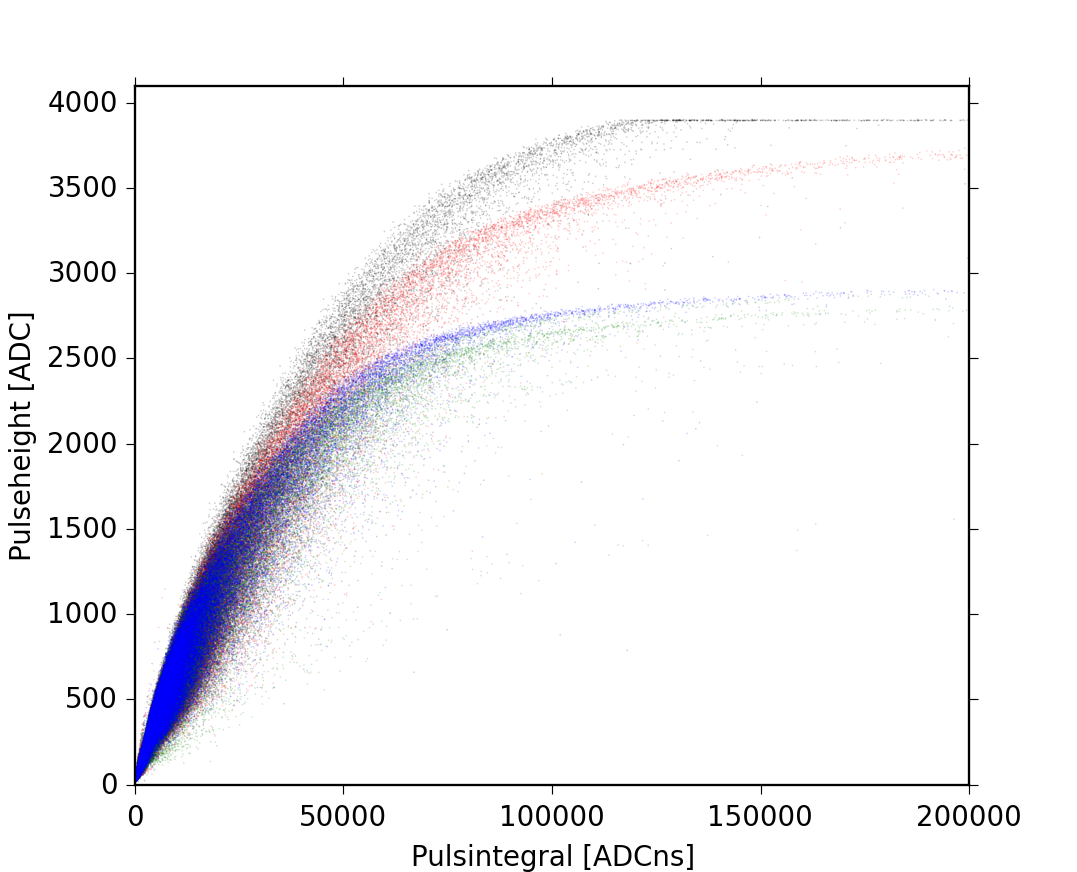
\includegraphics[width=0.6\textwidth]{plots/response/ph_vs_pi.png}
    \caption{\captitle{Pulseheight versus number of particles.}
             Indication of linearity of the \pmt.}
    \label{fig:transport_time}
\end{figure}


\subsection{PMT calibration}
\label{sub:pmt_calibration}

We created a setup where an optical fiber is connected to a cap which
directs the light at the window of a \pmt to send bursts of photons at
it. This is similar to a pulse generator, but with light. The pulses are
created by LEDs and produce short (\SI{20}{\nano\second}) pulses with an
intensity comparable to one or two \mip in a detector, making them
similar to real scintillator signals. The pulse intensity or efficiency
fluctuates \todo[inline]{upto 50\%? due to LED or PMT?}. However,
averaged over 100 samples the pulse is very consistent
\todo{size of fluctuations on averaged signal? small..}. A single fiber,
does not provide much control over the mean intensity and duration of
the pulses.

The setup provides 24 optical fibers, each with its own LED and slightly
different intensity. There are two caps that can be placed on a \pmt.
One cap allows for a single fiber to be connected while another contains
a bundle of many fibers allowing all, or a subset of, 24 fibers to be
used simultaneously. When using the bundle of fibers each fiber looses about
\SI{25}{\percent} signal strength due to the fiber-to-fiber connection.
Signals of over \SI{5}{\volt} are possible with the bundle of fibers.

Since April 2014 each \pmt that is going to be used for a \hisparc
detector is first tested in the LED setup suing a single fiber to ensure
it responds properly to light and that there is no significant
background noise. The test tries to find the voltage at which the pulses
have a pulse height around \SI{340}{\milli\volt}. This pulse height
value requires a voltage close to the normal operational voltage of
\pmts on a \hisparc detector.


\subsection{Measured linearity}

In an EAS many more than one particle may pass through a detector. The
response of the \pmt to higher signals needs to be investigated to
determine the accuracy with which multiple particles can be
reconstructed. To increase the intensity multiple fibers can be combined
using the bundle of fibers. The setup is shown in \todo{add nice
photo/schematic of setup}. Each fiber is tested separately to determine
its mean intensity, then different combinations of multiple fibers are
combined as input. The expectation is that the individual intensities of
the fibers are simply added together. However, a \pmt might become
saturated or less efficient for larger signals, being unable to supply
enough current.

There are several types of \pmt being used in the \hisparc experiment.
Most established stations used \pmts that were fully created by outside
manufacturers. However, several batches have been encountered where the
failure rate of the \pmt power supplies was high, the tubes were still
working fine. The costs to have the power supply replaced were
excessive. The \nikhef Electronics department, which also developed the
\hisparc electronics, have worked on \pmt power supplies for the \kmnet
neutrino telescope experiment. The \kmnet \pmts have other requirements
than those used for \hisparc so some modifications were required. The
\kmnet design has been modified to be suitable for \hisparc. There have
been a couple of iteration of the \hisparc \pmts. Multiple \pmts of each
of these versions have been tested.

The tests show that the new \nikhef produced \pmt power supply can
supply enough current to saturate the \hisparc electronics. Moreover
they have a lineair response curve. The output corresponds to the sum of
the inputs. The old power supplies are lineair up to \SI{1}{\volt}
(depending on voltage). At higher signals they start showing diminishing
returns, barely reaching \SI{2.2}{\volt}. This effect can also be seen
for some \hisparc stations because the pulse height histogram does not
reach the maximum \adc value (minus the baseline). The following figure
shows the test for a SensTech \pmt with its original power supply. Along
the x-axis are the expected pulse heights, determined from the sums of
individual fiber tests. The y-axis is the measured pulse height for
certain combinations of fibers.

\begin{figure}
    \centering
    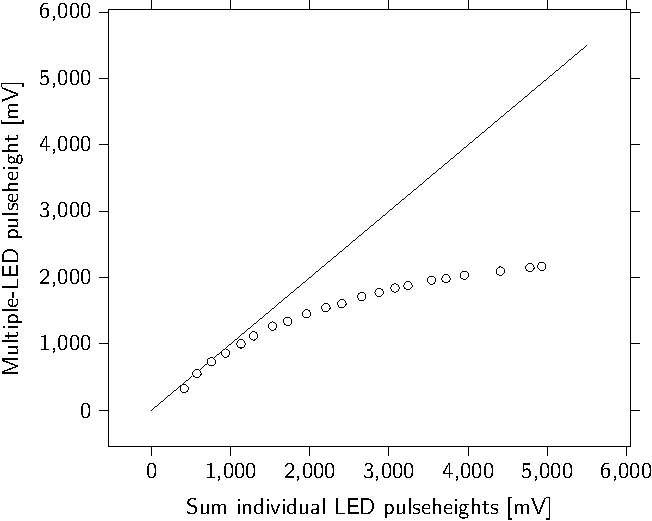
\includegraphics{plots/calibration/linearity_senstech_ph}
    \caption{Measurements of the pulse height linearity. Using a
             SensTech \pmt.}
    \label{fig:linearity_senstech_ph}
\end{figure}

The data is fit with the following function, as described in
\cite{icecube:pmt}.

\begin{equation}
    \ln V_{\mathrm{in}} = \ln V +
                          \frac{p_0 \left(\frac{V}{p_1}\right)^{p_2}}
                               {\left(1 - \frac{V}{p_1}\right)^{\frac{1}{4}}}
\end{equation}

The parameters have no physical meaning.


From the detector data can already see non-linearity by plotting the
measured pulse heights against the pulse integrals for the same events
\todo[inline]{figure showing the ph v pi}. For the old \pmts this
already showed that the pulse height is not lineair. However, it does
not show if the pulse integral is lineair or not. By measuring the pulse
heights and integrals using the setup we can see show non-lineair they
both are.

\begin{figure}
    \centering
    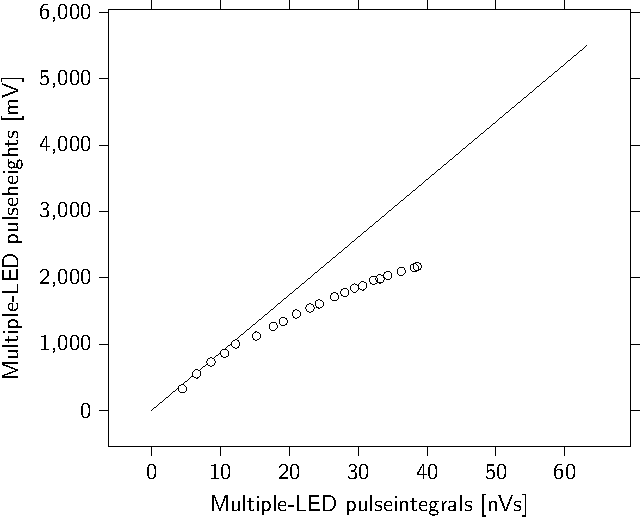
\includegraphics{plots/calibration/linearity_senstech_ph_pi}
    \caption{Measurements of the pulse height versus pulse integral.}
    \label{fig:linearity_senstech_ph_pi}
\end{figure}

The \adcs in the \hisparc electronics are designed and calibrated to
make the range \SIrange{200}{4096}{\adc} correspond to the range
\SIrange{0}{-2}{\volt}. Signals greater than \SI{-2}{\volt} are clipped,
preventing the pulse height to provide an accurate measure of signal
strength. The clipping also affects the pulse integral, however,
non-saturated parts of the signal still grow bigger, so the integral
continues to grow.

\todo{Using ND-filters to weaken the signal, to check for walk
      (arrival time determination).}
